\documentclass{beamer}
\usepackage[utf8]{inputenc}

\usetheme{Madrid}
\usecolortheme{default}
\usepackage{extarrows}
\usepackage{amsmath}
\usepackage{extarrows}
\usepackage{amssymb,amsfonts,amsthm}
\usepackage{txfonts}
\usepackage{tkz-euclide}
\usepackage{listings}
\usepackage{adjustbox}
\usepackage{array}
\usepackage{tabularx}
\usepackage{gvv}
\usepackage{lmodern}
\usepackage{circuitikz}
\usepackage{tikz}
\usepackage{graphicx}
\usepackage{amsmath} 

\setbeamertemplate{page number in head/foot}[totalframenumber]

\usepackage{tcolorbox}
\tcbuselibrary{minted,breakable,xparse,skins}

\definecolor{bg}{gray}{0.95}
\DeclareTCBListing{mintedbox}{O{}m!O{}}{%
  breakable=true,
  listing engine=minted,
  listing only,
  minted language=#2,
  minted style=default,
  minted options={%
    linenos,
    gobble=0,
    breaklines=true,
    breakafter=,,
    fontsize=\small,
    numbersep=8pt,
    #1},
  boxsep=0pt,
  left skip=0pt,
  right skip=0pt,
  left=25pt,
  right=0pt,
  top=3pt,
  bottom=3pt,
  arc=5pt,
  leftrule=0pt,
  rightrule=0pt,
  bottomrule=2pt,
  toprule=2pt,
  colback=bg,
  colframe=orange!70,
  enhanced,
  overlay={%
    \begin{tcbclipinterior}
    \fill[orange!20!white] (frame.south west) rectangle ([xshift=20pt]frame.north west);
    \end{tcbclipinterior}},
  #3,
}
\lstset{
    language=C,
    basicstyle=\ttfamily\small,
    keywordstyle=\color{blue},
    stringstyle=\color{orange},
    commentstyle=\color{green!60!black},
    numbers=left,
    numberstyle=\tiny\color{gray},
    breaklines=true,
    showstringspaces=false,
}
\title %optional
{10.7.81}


\author 
{Kartik Lahoti - EE25BTECH11032}

\begin{document}


\frame{\titlepage}
\begin{frame}{Question}
Two circles, each of radius $5$ units, touch each other at $\brak{1,2}$. If the equation of common tangent is 4x + 3y = 10, find the equations of circles.
\end{frame}

\begin{frame}{Theoretical Solution}

Let , 
\begin{align}
    \vec{P} = \myvec{1\\2}
\end{align}


Given Line, 

\begin{align}
    \vec{n}^{\top}\vec{x} = 10
\end{align}

Normal Vector $\vec{n} = \myvec{4 \\ 3}$

\end{frame}

\begin{frame}{Theoretical Solution}
Unit vector $\vec{u}$ in direction of $\vec{n}$

\begin{align}
    \vec{u} = \frac{\vec{n}}{\norm{\vec{n}}} = \myvec{\dfrac{4}{5} \\ \dfrac{3}{5}}
\end{align}

Let $\vec{O_i}$ be the center of Circles, then

\begin{align}
    \vec{O_i} = \vec{P} \pm 5\vec{u} \\ 
    \vec{O_i} = \myvec{1\pm4 \\ 2\pm3} 
\end{align} 


\begin{align}
    \therefore \vec{O_1} = \myvec{5 \\ 5} , \vec{O_2} = \myvec{-3\\-1}
\end{align}
\end{frame}

\begin{frame}{Theoretical Solution}
Equation of Circles are : 

\begin{align}
    O_1 \colon g\brak{\vec{x}} = \vec{x}^{\top}\vec{V}\vec{x} + 2\vec{u}^{\top}\vec{x} + f 
\end{align}

\begin{table}[H]
    \centering
    \begin{tabular}[12pt]{ |c| c|}
    \hline
    \textbf{Points} & \textbf{Name}\\ 
    \hline
	\myvec{7\\10} & Point $\Vec{A}$ \\
    \hline 
	\myvec{-2\\5} & Point $\Vec{B}$\\
    \hline
	\myvec{3\\4} & Point $\Vec{C}$\\
    \hline
\end{tabular}
    \caption{1}
    \label{tab:placeholder}
\end{table}
\end{frame}
\begin{frame}{Theoretical Solution}
\begin{align}
    O_2 \colon g\brak{\vec{x}} = \vec{x}^{\top}\vec{V}\vec{x} + 2\vec{u}^{\top}\vec{x} + f 
\end{align}

\begin{table}[H]
    \centering
    \begin{table}[h!]
    \centering
    \begin{tabular}{|c|c|c|}
        \hline
        Point & For $k=3$ & For $k=-\tfrac{9}{2}$ \\
        \hline
        $A$ & $\myvec{1\\-1}$ & $\myvec{1\\-1}$ \\
$B$ & $\myvec{-4\\6}$ & $\myvec{-4\\-9}$ \\
$C$ & $\myvec{-3\\-5}$ & $\myvec{\tfrac{9}{2}\\-5}$ \\
        \hline
    \end{tabular}
    \caption{Vertices of $\triangle ABC$ after substituting $k$ values}
    \label{tab:triangle_values}
\end{table}

    \caption{2}
    \label{tab:placeholder}
\end{table}
\end{frame}

\begin{frame}{Plot}
    \centering
    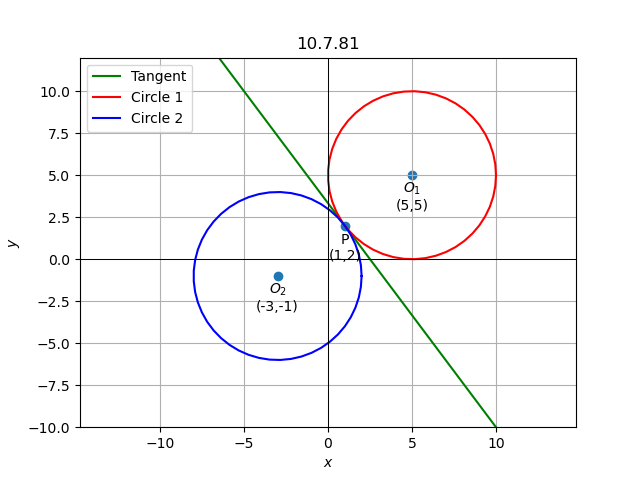
\includegraphics[width=\columnwidth, height=0.8\textheight, keepaspectratio]{../figs/graph2.png}   
\end{frame}

\end{document}
